% This is LLNCSDE2.TEX, a variation of LLNCS.DEM
% (the demonstration file of
% the LaTeX macro package from Springer-Verlag
% for Lecture Notes in Computer Science,
% version 2.2 for LaTeX2e),
% which can be used by volume editors for the preparation
% of the front matter pages and the author index
%
% Last changes: 04.08.1999, Antje Endemann (endemann@springer.de)
%
%%%%%%%%%%%%%%%%%%%%%%%%%%%%%%%%%%%%%%%%%%%%%%%%%%%%%%%%%%%%%%%%%%%%%
% In order to generate an Author Index do the following:
% After TeXing this document start the program MakeIndex by typing
% MAKEINDX -S SPRMINDX.STY <filename>
% (generates an IND file for the Author Index)
% into the DOS command line.
% (At other systems you may have to use the command MAKEINDEX.)
% Now TeX this file once again, then you will get an Author Index.
% TeX this file once more, then the TOC will be complete.
%%%%%%%%%%%%%%%%%%%%%%%%%%%%%%%%%%%%%%%%%%%%%%%%%%%%%%%%%%%%%%%%%%%%%

\documentclass{llncs}
%\usepackage{ucs}
\usepackage[utf8]{inputenc}
\usepackage{fancyhdr}
\usepackage[dvips]{graphicx}
\usepackage{graphicx}
\usepackage{fancyhdr,epsfig}
\usepackage{a4wide}
\usepackage{amssymb}
\parskip 3ex



\begin{document}

\title{A comprehensive design model for integrating
learning  processes in e-learning context-aware web applications}

\author{Alejandro Sartorio\inst{1,3}, Griselda Guarnieri\inst{1,2}, Guillermo Rodriguez\inst{1,3}, Patricia San Martin\inst{1,2}}

\index{Ekeland, Ivar}
\index{Temam, Roger}
% use the command \index{<name>} for index entries

\institute{UNR Universidad Nacional de Rosario \and CONICET \and  Agencia}

\maketitle


\begin{abstract}
Web applications have evolved from simple read-only e-learning websites to
complex data- and operation-intensive systems. The main goal of this kind of
application is to provide the users with services (throught the tools as wiki, forum, lessons, etc.) that assist them in carrying out activities according to a given set of pedagogical rules. The addition Obra Abierta requirement to e-learning web applications poses new challenges, such as the managing the
interplay between pedagogical process execution and navigation, and improving
the user’s experience in accessing the services that the e-learning web application offers.
This paper presents a comprehensive design model for integrating pedagogical
processes in e-learning applications focused in the relation between essential object entities (in this case, Students, Teachers and Tools).The model is based on DRObAb, an extended
and revised version of the Ubiquitous Web Applications (UWA) Transaction
Design model for designing web transactions. UWAT+ROA makes it possible to
design e-learnig web application pedagogicaltransactions according to the user’s context and to
integrate the e-learnig web transaction design with the information and navigation design
of the web application.
\end{abstract}


\section{Introducción}

Este trabajo presenta un diseño compresivo para el modelado de los procesos de educación e investigación (PEI) en un dispositivo hipermedial context aware dinámico (DHc-aD). El modelo está basado en UWAT+ (Distante, 2004), una versión extendida y adaptada de UWA Transaction Design Model para el diseño de transacciones en aplicaciones Web  


Desde el punto de vista de la ingeniería de software, desatender o resolver incorrectamente la documentación para el diseño de procesos de educación e investigación pueden causar numerosos prolemas reflejados en el proceso de configuración  de un DHc-aD. Estos problemas pueden ser:


..hay diferentes tipos de modelos, nosotros nos centraremos en las extensiones para poder implementar la teoríade coordinaciń de contratos...
\begin{itemize}


 \item Dificultades en la comunicación y entendimiento entre el diseñador y el demandante (en este caso de estudio, expertos pedagógicos e instituciones respectivamente).
 \item Determinación de las relaciones donde se justifique la inclusión de contratos. 
 \item Visualización y caracterización de la conformación de las "redes" de apendizajes e investigación en el dispositivo \footnote{ nota al pié sobre redes de aprendizaje}.


..... Teniendo en cuenta nuestra experiencia en el trabajo multidiciplinario de Obra Abierta

..... En este trabajo se retoma el modelo UWAT+ con pequeñas modificaciones 

..... con un pequeño agregado para la extensión del modelo 



\end{itemize}


....... referenciar a que tipo de modelo corresponde este modelo.

.......  a través de este trabajo mostraremos un simple ejemplo para ilustrar las caractéristicas del modelo de diseño DRObAb 

.......  muy importante para la gente blanda tener un modelo de esta características

....... proponemos una adaptación de la definiciones de colección, slots, etc para educación 

\section{Documentación de los procesos de educación e investigación}


!!!!!!!! Pato rehacer y completar cada párrafo.....


Las transacciones en un DHc-aD están definidas como secuencias de actividades asociadas con un flujo de ejecución que permite al usuario desempeñar una determinada tarea  y/o alcanzar una meta a través del dispositivo hipermedial. Entoces, un porceso de educación e investigación puede ser interpretada como una especificación del concepto de "workflow" en un dispositivo hipermedial context-aware; con las reglas, normar y restricciones  subyacentes del proceso de enseñanza y aprendisaje......


Las transacciones en un DHc-aD  están formados por un conjunto de operaciones simples o complejas sobre datos y contenidos para la confección de un dispositivo hipermediale context-aware. Un ejemplo de un PDI, como se verá más adelante, la intervención de un alumno en un espacio de edición colaborativa.....

Las transacciones en un DHc-aD son el camino para la representación de los PEI y proveer a los usuarios de servicios, accediendo a través de las herramientas que los contienen (wiki, fotro, video conferencia, taller, blog, etc.) La ejecución de transacciones de un DHc-aD supone tanto la navegación a través de las herramientas (por medios de los links de las componentes hpermediles) y el uso de sus servicios. Un ejemplo de servicio puede ser en una video conferencia, la posbilidad de que un alumno participe en un espacio de edicción colaborativa.

El diseño de las transacciones pueden abarcar varios niveles de abstracción y distintos formalismos pueden ser usados para su representación y documentación. Al menos tres nivels de abstracción pueden ser usados: (1) nivel conceptual, (2) nvel lógico, y (3) nivel de implementación.  El diseño conceptual permite una representación del sistema (las transacciones) 


los cuales pueden ser representados por 



Distintos formalismos y abstracciones pueden ser usados para la la representación de 

Web Transaction design can be accomplished at several levels of
abstraction and several formalisms can be used to represent and
document each of them. At least three levels of abstraction can be
used: (1) conceptual level, (2) logical level, and (3)
implementation level. The conceptual design gives a
representation of the system (the Web Transaction in our scope)
as perceived by the user and removed from implementation
issues. The implementation design focuses on providing the
system developers with all the specifications needed for realizing
the single components of the system. The logical design is a
middle level of abstraction design intended to translate the usercentered
specifications of the conceptual design into terms of
specifications closer to the implementation issues..



\section{Diseño de los temas}

Al igual que en las aplicaciones Web convencionales, el diseñador debe tener en cuenta algunas cuestiones conceptuales que deben ser concideradas en la etapa del disenho de un espacio hipermedial context aware para la investigación y el aprendizaje. En este sentido para el proyecto "\textit{Participar en Obra Abierta}" \cite{libro7} estuvieron presentes las siguientes consideraciones:

\begin{description}


\item DT1 - Los usuarios destinatarios se conformarán de: Graduados universitarios en Carreras vinculadas al campo audiovisual interactivo. (Artísticas, Comunicación Social, Tecnologías de Sonido y Multimedia, Ciencias de la Computación, Ingeniería de Sistemas, Arquitectura y Diseño, Ciencias de la Educación). Graduados, Docentes e Investigadores que estén relacionados con problemáticas de integración de las de las TIC en los procesos de enseñanza y aprendizaje en el contexto físico-virtual que desarrollen sus tareas en Instituciones de Nivel Superior.

\bigskip

\item  DT2 - Los participantes trabajando en grupos interdisciplinarios de acuerdo a su especialidad y sus perfiles profesionales deberán realizar:
Un diseño e implementación grupal a nivel prueba de laboratorio, de un taller físico-virtual para realizar un proyecto de obra que incluya una “demo” de un material hipermedial para el campo audiovisual interactivo que pueda ser utilizado en educación y/o investigación.

\bigskip

\item  DT3 - Para las introducciones conceptuales tendremos en cuenta los preconceptos, los prejuicios, los supuestos básicos y formación operativa en tecnologías informáticas de los destinatarios.  La reflexión y discusión de los distintos temas tratados la plantearemos bajo la metáfora de la mesa de arena, a partir de producciones o exploraciones analíticas realizadas en pequeños grupos interdisciplinarios utilizando las herramientas de comunicación hipermediales como por ejemplo, “Agora” de Sakai, que el dispositivo brinda. La utilización de dicha tecnología es constitutiva también al contenido del curso, cumpliendo una doble función: como soporte para la actividad de enseñanza, aprendizaje o investigativa en el contexto físico-virtual y como introducción a la problemática de los dispositivos hipermediales context-aware dinámico.

\bigskip
\item DT4 - Conocer, explorar y utilizar las posibilidades de los dispositivos hipermediales context-aware dinámicos y las herramientas disponibles en el desarrollo de procesos educativos, investigativos y de producción aplicados al campo audiovisual interactivo.

\bigskip
\item DT5 - Desarrollar y presentar una propuesta analítica sobre la participación  y producción textual en dichos dispositivos, adhiriendo o confrontado con lo planteado por el equipo de I$+$D Obra Abierta.

\bigskip

\item DT6 - Interpretar y debatir la perspectiva ético - filosófica de las comunidades de desarrollo de software libre y la calidad de los resultados de producción y transferencia de los desarrollos relacionados al campo audiovisual interactivo.

\bigskip
\item DT7 - Construir y aplicar herramientas analíticas a producciones hipermediales posibles de ser utilizadas en procesos educativos o investigativos, participando en una  Mesa de arena.

\bigskip

\item DT8 - Diseñar dispositivos hipermediales para educación, investigación y/o producción, utilizando el contrato como pieza de software, en el marco de la perspectiva contex-aware dinámico.

\bigskip
\item DT9 - Modalidad físico-virtual: El taller integrador tendrá 3 encuentros de 4 hs cátedra de duración en la institución a lo largo del cuatrimestre con el responsable general y/o el grupo responsable. En el contexto virtual tendrá diseñadas semanalmente actividades sincrónicas de 2 hs. (grupales de producción), un espacio de consulta de 1 hora (optativo) y actividades asincrónicas.
\end{description}



se deben considerar explicitamente  para el disenho de espacios hipermediales context aware dinámico \cite{libro} se debe tener en cuenta 


\section {Requerimientos para el diseño de procesos de aprendizaje-enseñanza-investigación}

!!!!!!!!!!!!!! ingresar un párrafo sobre procesos de aprendizaje-enseñanza-investigación

.... basado en la experiencias recogidas en Obra Abierta, fueron seleccionadas un conjunto de requerimientos bajo una metodología conveniente y se ha determinado un modelo de diseño de los procesos de ensenhanza-aprendizaje-investigación (PdEAI).  A continuación, se formalizan una serie de requerimientos contextualizados por una lista de temas y concideraciones que se debe satisfacer en un espacio ideado por medio dispositivo hipermedial context-aware dinámico.    

\begin{description}
\item Req1 - Identificación de las herramientas que se utilizarán en el proceso de aprendizaje.

\bigskip
\item Req2 - Identificación de los elementos para el disenho hipermedial utilizados como contenidos por las herramientas (según Req1).
\bigskip
\item Req3 - Descripción y caracterización del flujo de desplazamiento enunciativos (FDE).
\bigskip
\item Req4 - Definir y utilizar (instrumentalmente) los estados en el aprendizaje.

\bigskip
\item Req5 - Descripción y caractericación de la información de contexto que condicione (influya) en los ateriores requerimientos (Req1, Req2, Req3 y Req5).

\bigskip
\item Req6 - Descripción del rol de dos o más usuarios (pertencientes a miembros en formación y grupos responsables) intervien en un determinado proceso de aprendizaje. 

\bigskip
\item Req7 - Definir cuales elementos pertencecientes a los learning object (LO) son afectados en las distintas actividades (procesos) \cite{libro5}

\bigskip
\item Req8 - Identificación de las relaciones (Objetivo-Objetivo) que ameriten su implementación a través de un contrato context-aware.

\end{description}

Pese a no ser exhautivo, el listado de requerimientos es representativo en cuanto a las necesidas básicas que se deben atender en en los PdEAI en un espacio hipermedial contex-aware. Su definición (caracterización) es resultado de la investigación del grupo Obra Abierta donde se conjugan, los esfuerzos realizados para concretar una correcta abstracción de los requerimientos resueltos conceptualmetes (filosófica, pedagógica, sociológia y psicologicamente)\cite{pato1} que a su vez pueden ser transformadas (mediante una construcción semi-formal) para ser resueltas mediante un  modelo de diseño de requerimientos - forward, para este caso que nos ocupa - para nuestra propuesta sistema adaptado para aplicaciones Web colaborativas.

La Tabla \ref{di_re} muestra como se encuedran cada una de los temas identificados el la sección \ref{disenotemas} dentro de los requerimientos anteriormemte establecidos.	

\begin{center}
\begin{tabular}{l l }
\hline
\textit{\textbf{Especificación de Temas}\textit{}                      -}& \textit{\textbf{Caracterización de Requerimientos}}\\
\hline
DT1  				& Req4, Req5, Req6 \\
DT2				& Req1, Req2, Req3, Req4, Req5, Req6, Req7, Req8 \\
DT3				& Req4, Req5, Req6 \\
DT4				& Req1, Req8 \\
DT5				& Req3, Req7, Req8 \\
DT6				& Req3, Req6, Req7, Req8 \\
DT7				& Req1, Req3, Req5, Req8 \\
DT8				& Req1, Req2, Req3, Req4, Req5, Req6, Req7, Req8 \\
\hline

 \end{tabular}  
\end{center}

\section {Diseño de procesos de enseñanza-aprendizaje-investigación con DRObAb}


En esta sección se describen los resultados de la apliación de DRObAb para el espacio dedicado al libro "Hacia un dispositivo hipermedial contex-aware" (San Martín P, et. al) \cite{libro}.  Este  modelo fue aplicado parcialmente para el diseño de los requerimientos fundamentales y el modelado del compertamiento funcional enmarcado bajo la perspectiva de Obra Abierta \cite{ObraAbierta}. Se identificarán las t




El diagrama de la figura \ref{procesodiseno} muestra una adaptación del diseño de procesos de UWA \cite{UWA} que se utiliza en DRObAb para el diseño de los PdEAI. Para ilustrar el proceso de diseño es IDEF0 (IDEF-0, 1993). A continuación, se decriben las fases que fueron adoptadas en cuya implicancia se determinen las cuestiones que involucran a los contratos y la caracterización de los PdEAI significativos de Obra Abierta para \cite{libro7}:

\begin{enumerate}
 \item Determinación de Requerimientos 
 \item Diseño de procesos
 \item Diseño de operaciones
 \item Diseño de navegación
\end{enumerate}



	\begin{figure}[!h]
        \begin{center}

	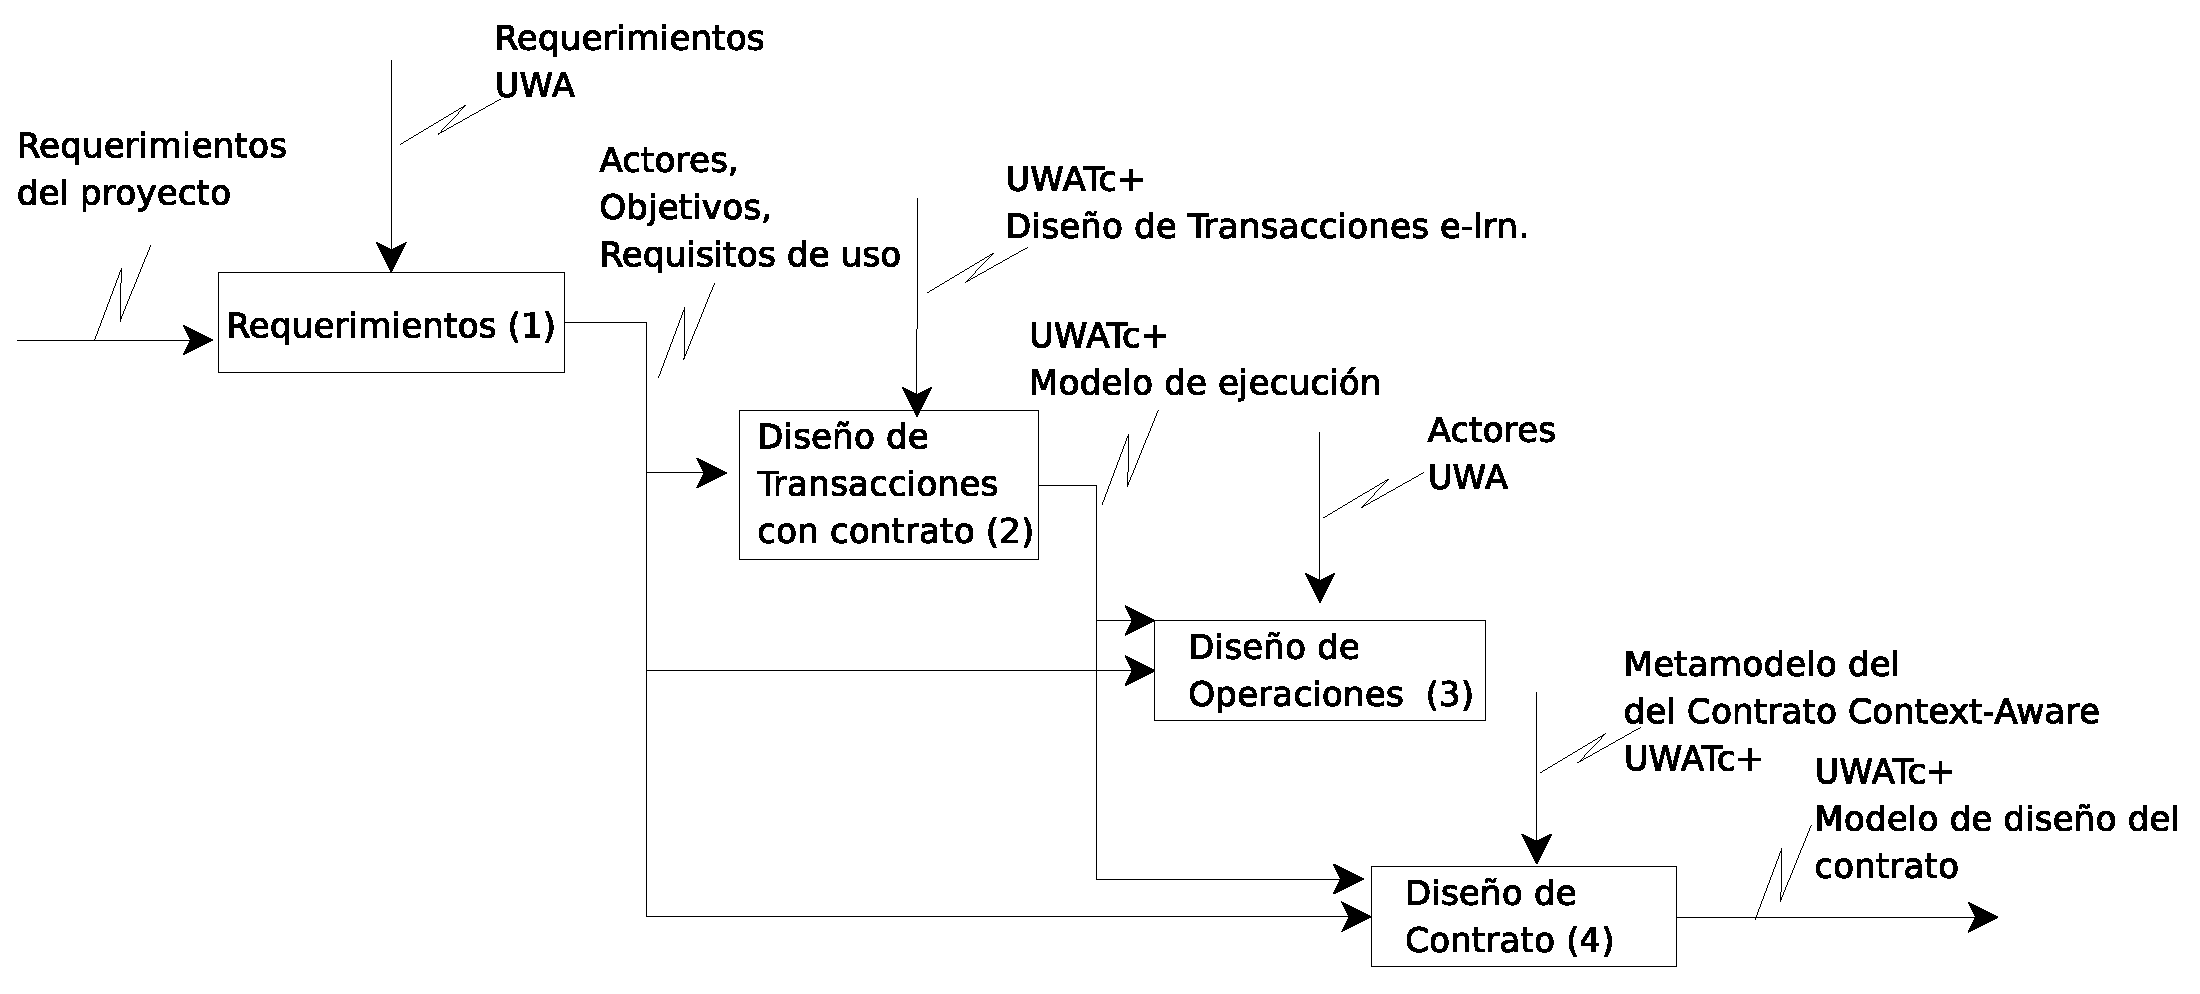
\includegraphics[width= 4 in,totalheight=1 in]{procesodiseno.eps}
	\caption{\small \sl El proceso de diseñar PdEAI en un dispositivo ipermedial context-aware con DRObAb} \label{proceso de diseno}
         \end{center}
         \end{figure}


\subsection{Determinación de Requerimientos} \label{sdr}

La fase de Determinación de Requerimientos toma como entrada las especificaciones del proyecto y produce, por medio de un mecanismo de refinamiento, las siguientes salidas:
\begin{itemize}
 \item  Cada actor con su objetivos relativos.
 \item  Los requerimientos para el dispositivo hipermedia.
\end{itemize}
 
El modelo utilizado es orientado a objetivos: cada actor se identifica con al menos un objetivo, i.e, una abstracción de los objetivos que a través del dispositivo hipermedial se debe alcanzar; cada objetivo es refinado en otros sub-ojetivos, concretando hasta poder definir el requerimiento objetivamente o en un bajo nivel suficiente para poder implementar el requerimiento. Este fase es similar a la descripta en (UWA Consortium, 2001) \cite{UWA}. 

Para este caso de uso, atendiendo a los lineamientos en \cite{libro7}, se descibe parte del modelo original donde se carateriza los objetivos involucrado con un actor relevante del sistema. A su vez, a medida que se van derivando los sub-objetivos comienzan a establecerse requerimientos concernientes a la teoría de coordinación de contratos context-aware \cite{libro5,contratos}. En la figura \ref{requerimientos} dicha situación ocurre en la derivación de las tres ramas de objetivos y sub-objetivos, influyendo directamente en la composición de la componente contrato; tomando desde la \textit{\textbf{rama 1}} un servicio de una herramienta de un espacio de discusión (ejemplo, el foro), de la \textit{\textbf{rama 2}} se despenden las información necesaria para poder articular dicho servicio teniendo en cuenta la información de contexto y, luego, de la \textit{\textbf{rama 3}} aporta el consenso de los expertos (del dominio e-learning) para la inclusiñon de los contratos en aquellas relaciones que mantendrán las propiedades de un dispositivo hipermedial dinámico context-aware \cite{libro5}. De esta manera, te tienen todos los elementos (caracterizados y formalizados para su compresión) para la confección de los contratos context-aware.


	\begin{figure}[!h]
        	\begin{center}
		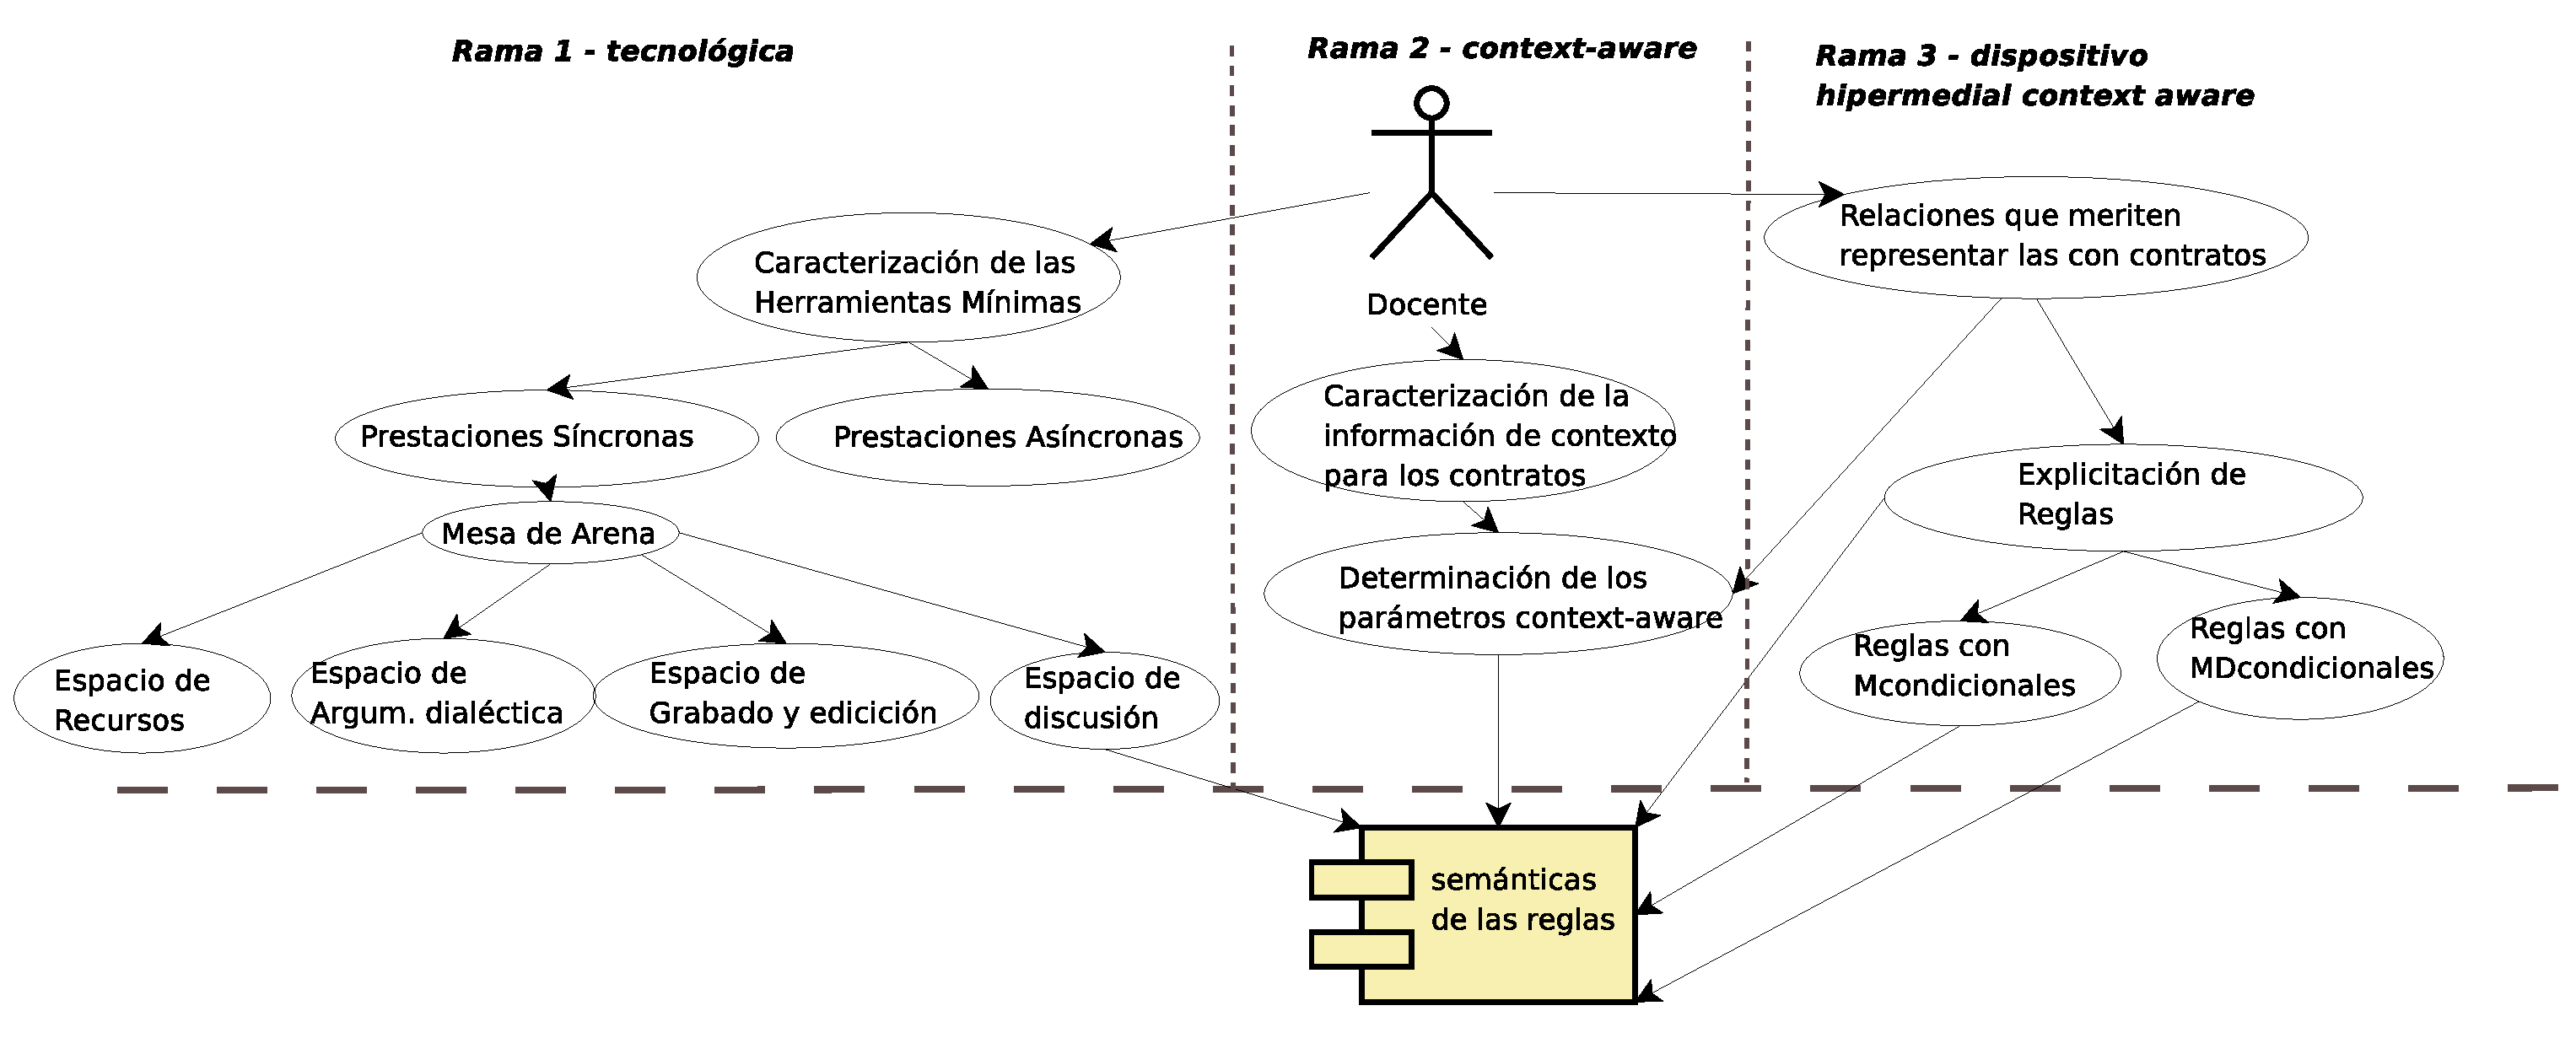
\includegraphics[width= 6 in,totalheight=3 in]{Requerimientos.eps}
                \caption{\small \sl Objetivos de al alto nivel  para el PdEAI} \label{requerimientos}
         	\end{center}
         \end{figure}


Non-contextual navigation is specied by dening the access schema, which con-
sists of a number of collections.
A collection [Garzotto et al. 1994] is a set of objects that may be used as a
meaningful index to the content of the application. Normally collections range over
(a subset of) the instances of a component (e.g., the set of professors in a Faculty's
site, the set of XVII Century paintings in a Museum's site). To allow hierarchical
indexes, they may also range over other collections (e.g., the collection of all painters
of a Museum may be substructured into the collection of XVI Century painters, of
XVII Century painters, and so on).



\subsection{Diseño del Procesos}

El diseño de procesos retoma la misma idea y modelo propuesto por UWA+ para el diseño de transacciones \cite{UWA+}. Partiendo de los resultados de los Requerimientos, fundamentalmente de la caracterización de los contratos, pueden ser seleccionados una series de procesos, i.e. objetivos que requieren la ejecución de una o más actividades para su cumplido. Para cada uno de los objetivos se deben ser diseñados procesos (el equivalente a las transacciones en UWA+), los cuales en principio deben ser establecidos desde un punto de vista estático (en este trabajo no abordaremos tal consideración) y luego, desde un punto de vista dinámico por medio de un modelo de ejecución de procesos. En la figura \ref{ejecucion de procesos} se muestra una porción del modelo de ejecución de un PdEAI en donde se usa el contrato modelado en la fase de Determinación de Requerimientos (figura \ref{requerimientos}, sección \ref{sdr}). 

por q tomamos la parte dinámica y no la estática

En la figura \ref{proceso}


\begin{figure}[!h]
        \begin{center}

	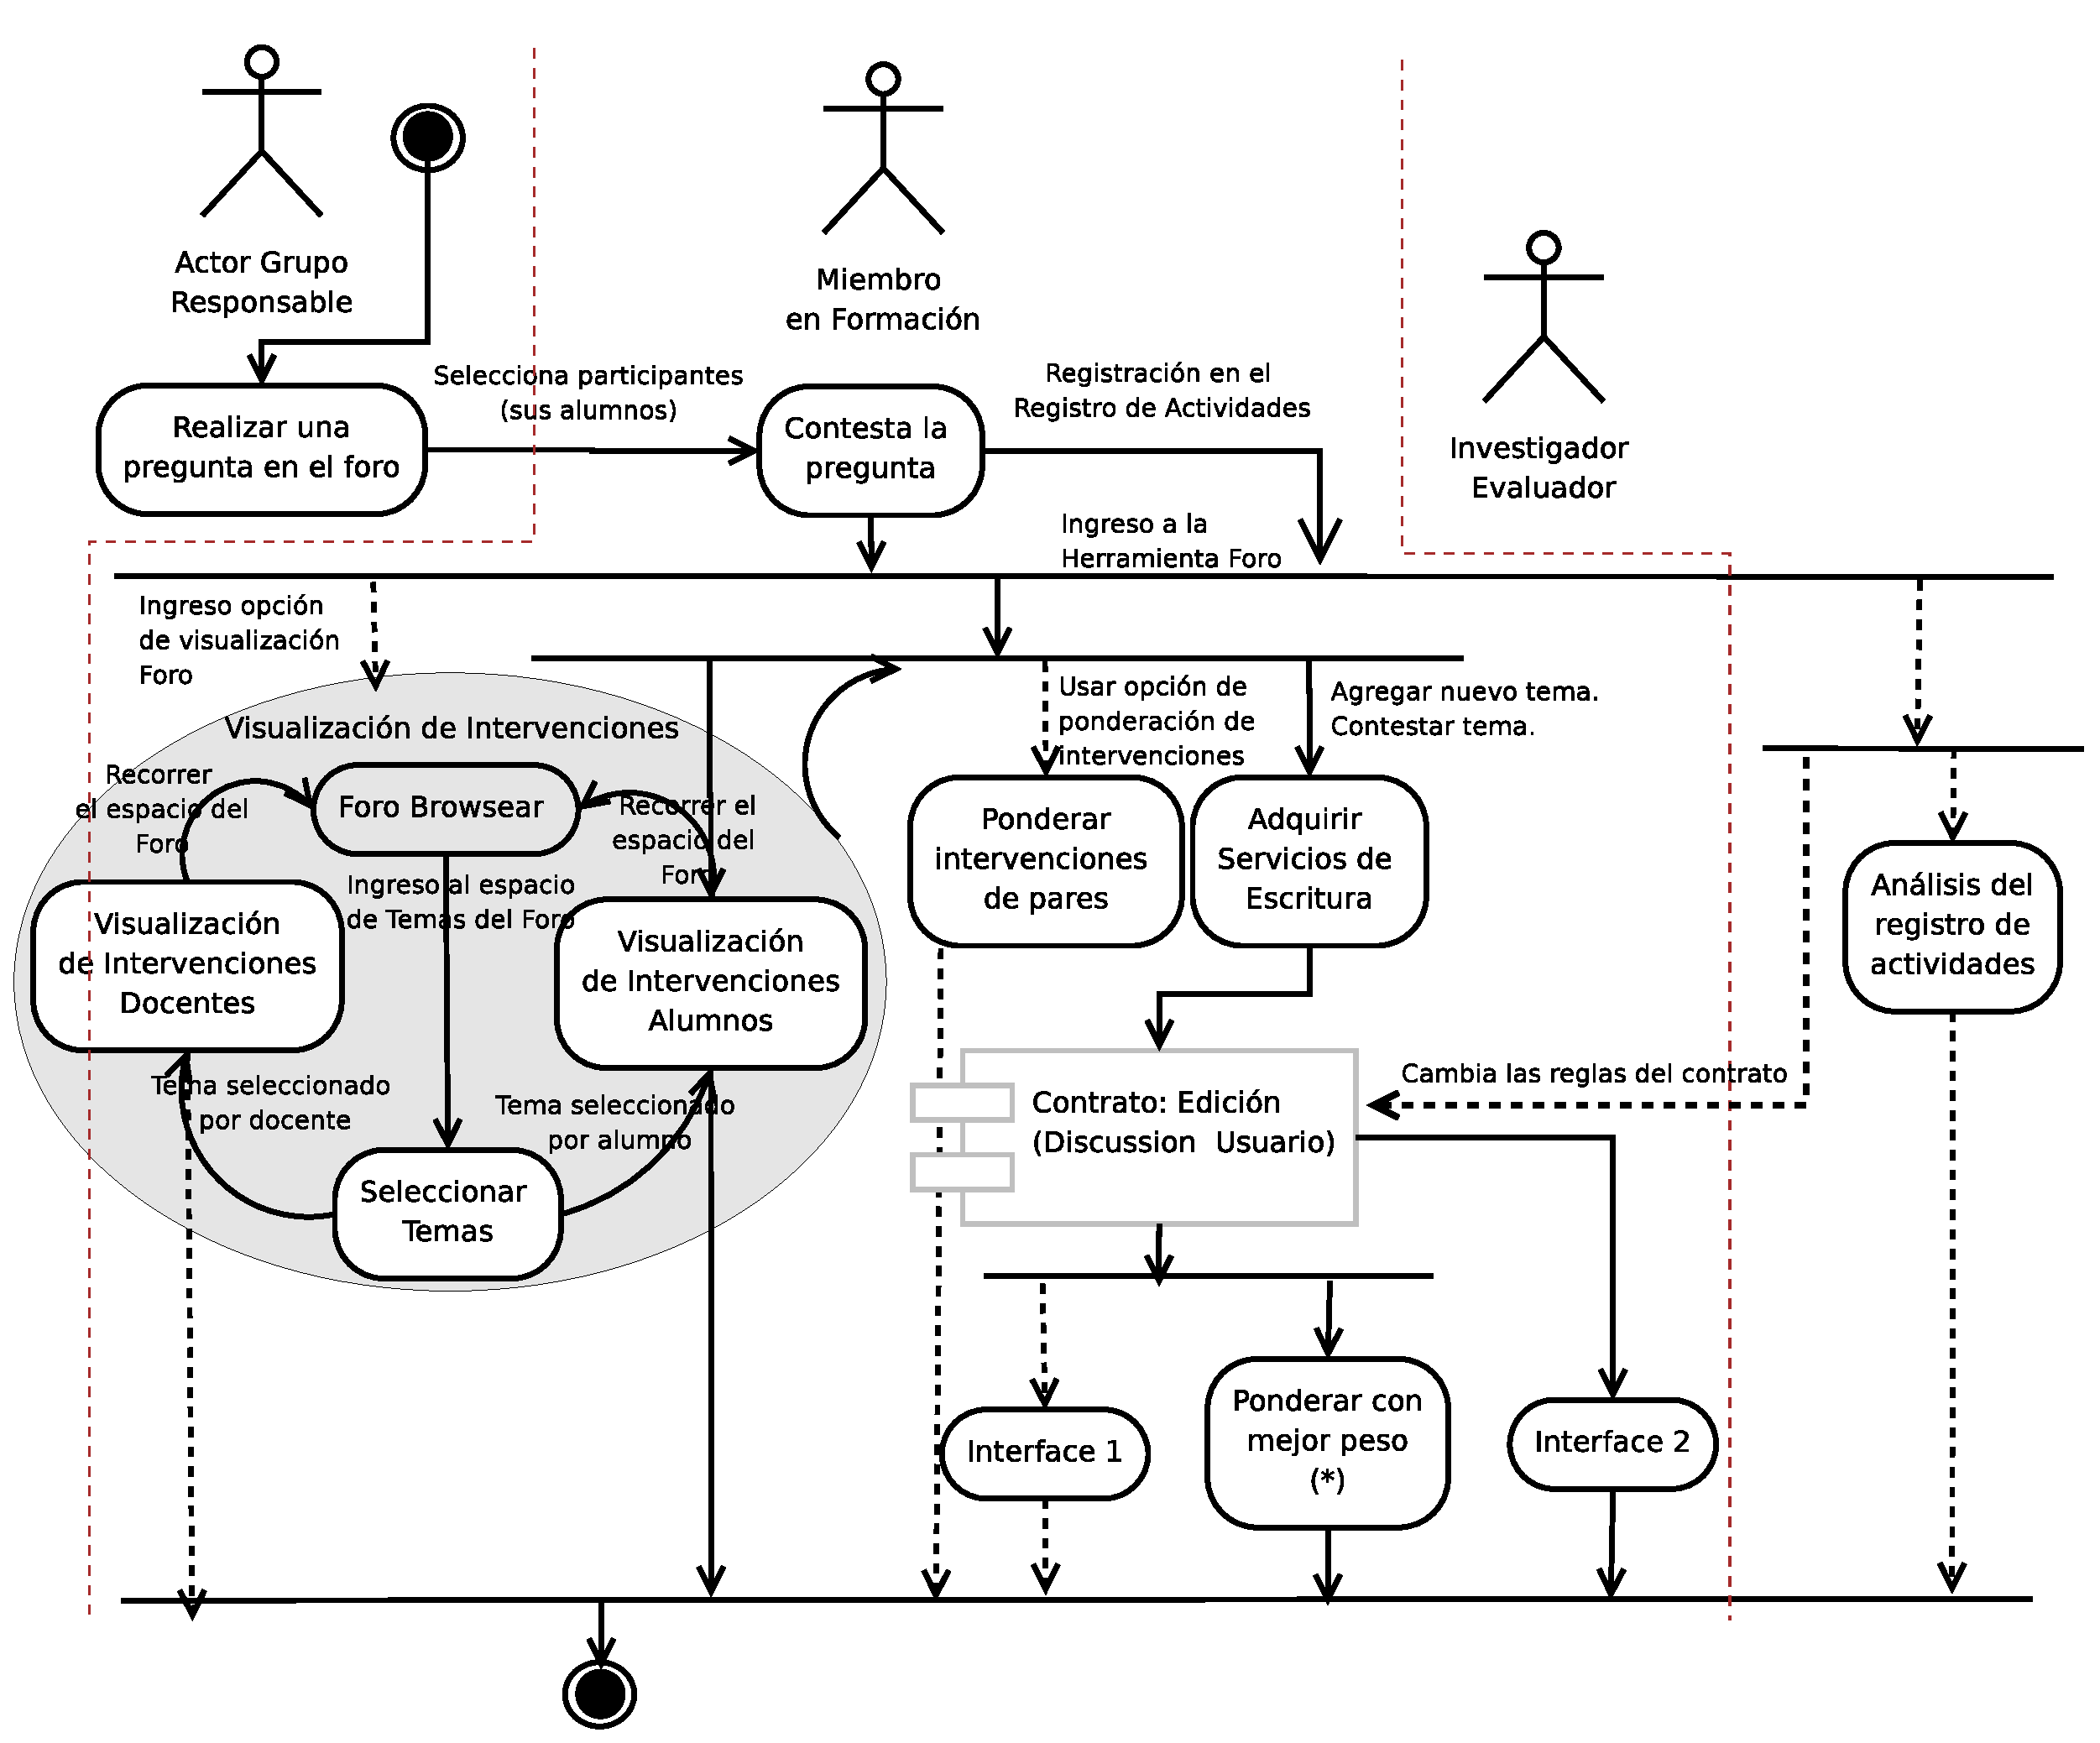
\includegraphics[width= 5 in,totalheight=3.5 in]{proceso.eps}
                                    \caption{\small \sl Modelo de ejecución de Procesos de Educación e investigación} \label{proceso}
         \end{center}
         \end{figure}



\subsection{Diseño de Operaciones}

\section{Modelo Relacionados}

Si bien no se tiene referencia sobre modelos de diseño específicos para aplicaciones e-learning al estilo de los dispositivos hipermedial context-aware dinámico, nuestra propuesta de DRObAb está inspirada en los aportes sobre diseño  

\subsection{UWA}
\subsection{OOHDM}
\subsection{WSDM}
\subsection{UWE}
\subsection{UWA}
\subsection{WebML}

 \begin{center}\begin{tabular}{cccccc}
  & &  \multicolumn{3}{c}{Métodos} \\ 
 Requerimiento & UWA &  OOHDM &  WSDM &  UWE & WEBML \\ 
 \hline 
 20 &  \multicolumn{1}{l}{23} &  34 &  \multicolumn{1}{l}{56} & 87 \\ 
 \cline{2-2} \cline{4-4} 
 25 &  22 &  56 &  76 & 23 \\ 
 \hline 
 \end{tabular}\end{center} 
 
\section{DRMObAb: una adaptación para el modelado de requerimientos para Obra Abierta}


%-------------------------  bibliografía ----------------------------------


\newpage

\begin{thebibliography}{1}

\bibitem{libro5} Sartorio A., San Martin P., 2007. {Sistemas Context-Aware en dispositivos hipermediales dinámicos para educación e investigación}

\bibitem{libro} San Martín P., Sartorio A., Guarnieri G., De la Riestra M., 2007. {Hacia un dispositivo hipermedial context aware dinámico. Educación e Investigación para el campo audiovisual interactivo}

\bibitem{ObraAbierta} Sartorio A, San Martin P., 2007. {Sistemas Context-Aware en dispositivos hipermediales dinámicos para educación e investigación}



\end{thebibliography}


\end{document}
